\newcommand{\twominisw}[4]{\begin{figure}[H]
                \centering
		\begin{minipage}{#3\linewidth}
			#1
		\end{minipage}
		\begin{minipage}{#4\linewidth}
			#2
		\end{minipage}
              \end{figure}}
\documentclass{beamer}
\usetheme{polimi}
\graphicspath{{../figures/}}
% Usage instructions can be found at: https://github.com/elauksap/beamerthemepolimi
\usepackage[utf8]{inputenc}
\title{La detonazione come metodo propulsivo}
\subtitle{Perchè, come e gli ultimi sviluppi dei propulsori a detonazione rotante.}
\author{Lorenzo Pasqui, 10703226}
\date{\today}

\begin{document}

\begin{frame}
    \maketitle
\end{frame}
\begin{frame}
  \begin{itemize}
    \item   Lu, Frank K., and Eric M. Braun. "Rotating detonation wave propulsion: experimental challenges, modeling, and engine concepts." Journal of Propulsion and Power 30.5 (2014): 1125-1142.
    \item Teasley, Thomas W., et al. "Current state of NASA continuously rotating detonation cycle engine development." AIAA SciTech 2023 Forum. 2023.
    \item Shaw, Ian J., et al. "A theoretical review of rotating detonation engines." (2021).

  \end{itemize}
\end{frame}
\begin{frame}
  Se la velocità della combustione avviene a velocità inferiori a quella del suono si parla di \textbf{Deflagrazione}.
  \begin{figure}
    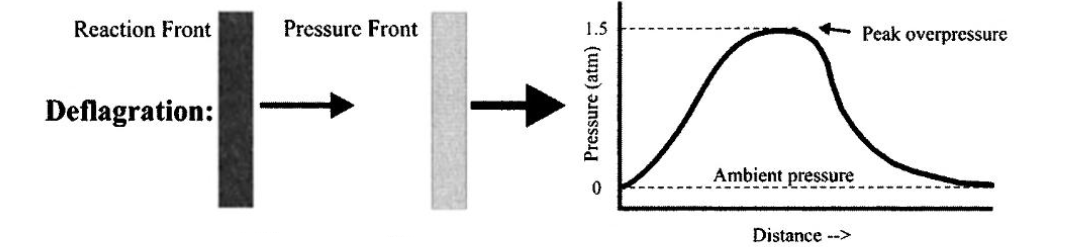
\includegraphics[scale = 0.4]{deflag_expl.png}
  \end{figure}
\end{frame}
\begin{frame}
Se la velocità della combustione avviene a velocità superiori a quella del suono si parla di \textbf{Detonazione}.
  \begin{figure}
    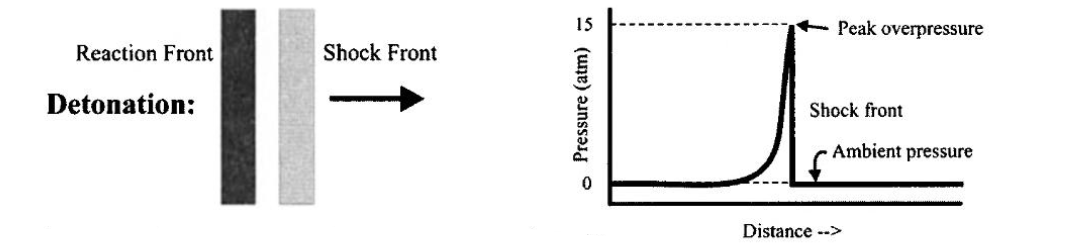
\includegraphics[scale = 0.4]{detonation_expl.png}
  \end{figure}
\end{frame}
\begin{frame}
  \twominisw{  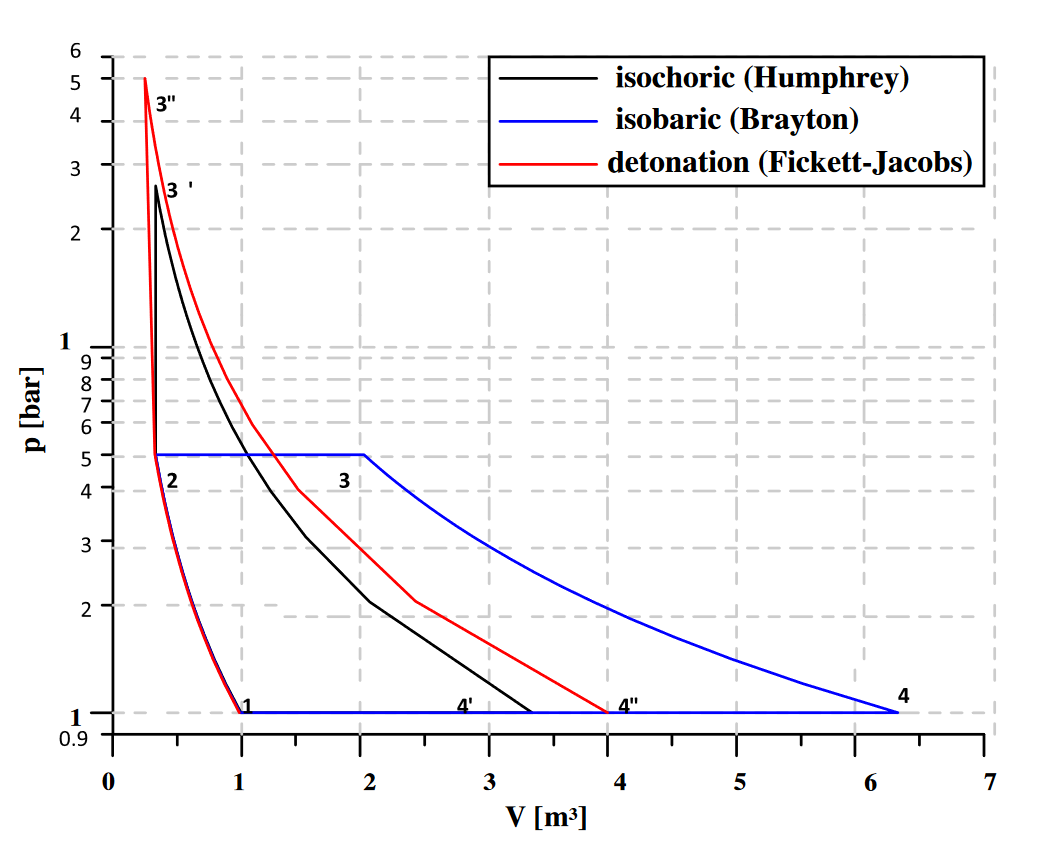
\includegraphics[scale=0.3]{Cicli Wolanski.png} 
  }{
  La maggior parte dei cicli termodinamici che utilizzano una deflagrazione seguono un ciclo Brayton (in blu). Se avviene una detonazione la turbina lavora in maniera quasi isocora e il ciclo termodinamico è quello di Fickett-Jacobs. Nel ciclo di Humphrey si suppone che la combustione avvenga a volume costante. 
}{.6}{.39}
\end{frame}
\begin{frame}
  \twominisw{
    \begin{gather*}
      \eta_B = 1 - \frac{1}{\left( \frac{p_2}{p_1} \right)^{\frac{k-1}{k}}} \\
      \eta_H = 1 - k \frac{T_1}{T_2} \frac{\left( \frac{T_{3^{\prime}}}{T_2} \right)^{\frac{1}{k}}}{\frac{T _{3^{\prime}}}{T_2} -1}\\ 
      {\eta}_{F} = 1 - k \frac{1}{ \left( \frac{p_3}{p_1} \right)^{\frac{k-1}{k}}} \frac{\left( \frac{T _{3 ^{\prime\prime}}}{T_2} \right)^{\frac{1}{k}}-1}{\frac{T _{3 ^{\prime\prime}}}{T_2}-1}
    \end{gather*}
  }{
    Come si può notare delle espressioni del rendimento per i diversi cicli, il ciclo di Fickett-Jacobs è il più efficiente.
  }{.5}{.45}
\end{frame}
\begin{frame}
  \begin{table}[h!]
       \begin{tabular}{|c | c | c | c | }
    	 \hline
    	 \textbf{Fuel} & \textbf{B (\%)} & \textbf{H (\%)} & \textbf{F (\%)}\\ 
    	 \hline\hline
    	 $ CH_4 $ &36.9 & 54.3& 59.3 \\ \hline
    	 $ H_2 $ &31.4 &50.5 & 53.2 \\ \hline
    	 $ C_2 H_2 $ &36.9 &54.1 &61.4 \\\hline
    \end{tabular}
  \end{table}
Nella tabella vengono calcolati per vari combustibili i valori di efficienza dei vari cicli termodinamici, per mettere in evidenza come il ciclo Fickett-Jacobs (J) sia il più efficiente se confrontato con i cicli Humphrey (H) e Brayton (B).
\end{frame}
\begin{frame}
  I primi utilizzi della detonazione come sistema propulsivo riguardano i propulsori ad onda di detonazione (PDEs). 
    \begin{figure}[H]
      \centering
      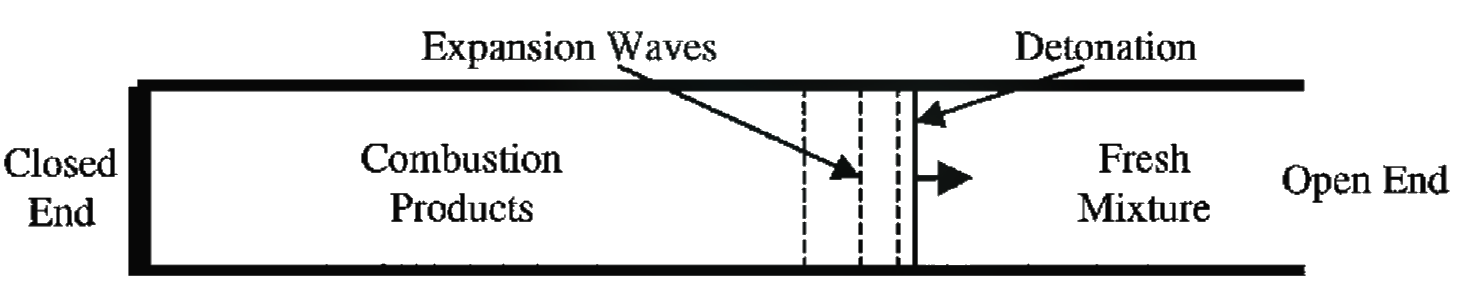
\includegraphics[scale=.2]{pde_scheme.png}
    \end{figure} 
    Nella camera di combustione viene immessa una miscela di ossidante e combustibile, che poi viene accesa. Il profilo di combustione è composto da una componente di deflagrazione, una fase transitoria da deflagrazione a detonazione e la detonazione.
\end{frame}
\begin{frame}
  \textbf{Problematiche dei PDEs}
  - Per ogni ciclo la camera deve essere liberata e la miscela reimmessa, limitando la frequenza dei cicli possibili ad ordini dei 100 Hz. Il che non solo abbassa l'efficienza del sistema propulsivo ma lo rende impraticabile per la propulsione, non approssimando sufficientemente una propulsione continua. In alcuni modelli per liberare la camera completamente dai prodotti della combustione residui che potrebbero influenzare il ciclo successivo, si raggiungono anche frequenze operative di circa 50 Hz. 
  - Le dimensioni della camera di combustione devono essere sufficienti per fare avvenire la transizione da deflagrazione a detonazione. Per ridurre le dimensioni è possibile mettere degli ostacoli per accelerare la transizione, ma questo riduce l'impulso specifico $ I _{sp} $.
\end{frame}
\begin{frame}
  Una soluzione alternativa è rimuovere la necessità di ripetere la transizione da deflagrazione a detonazione e riuscire ad alimentare e sostenere la reazione di detonazione. Partendo da questo approccio si giunge alla concettualizzazione dei propulsori a detonazione rotante.
\begin{figure}[H]
\centering
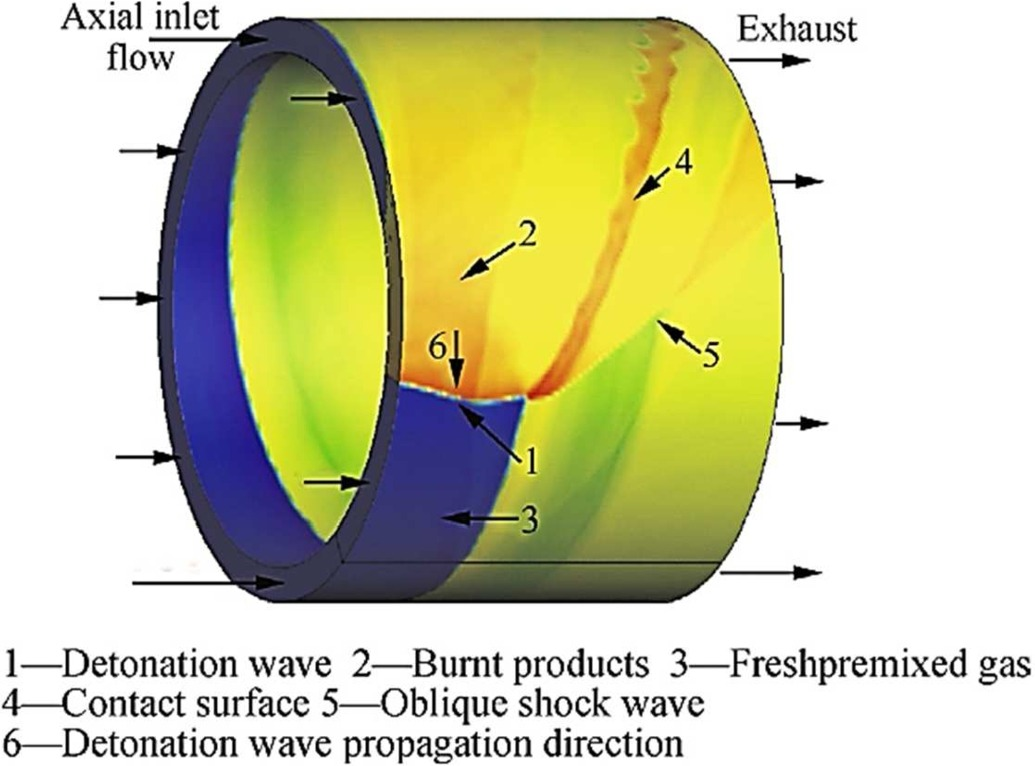
\includegraphics[scale=.6]{rde_intro.png} % https://www.sciencedirect.com/topics/engineering/rotating-detonation-engine
\end{figure}
\end{frame}
\begin{frame}
  \begin{figure}[H]
\centering
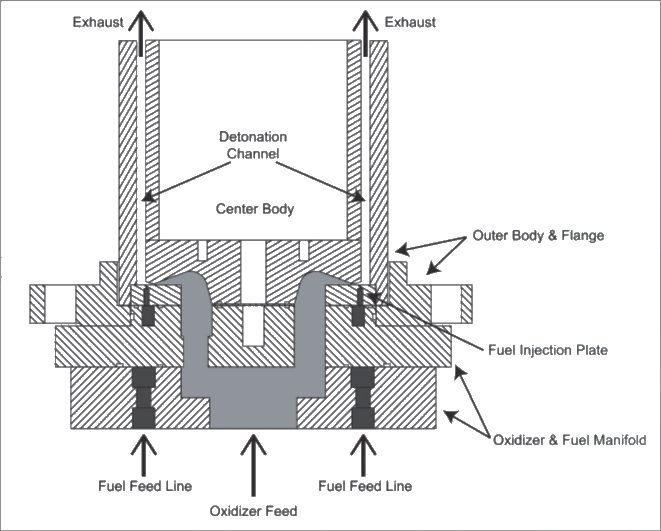
\includegraphics[scale=.2]{cross_rde.png}
\end{figure} 
\end{frame}
\end{document}
